\documentclass[runningheads,a4paper]{llncs}

\usepackage{graphicx}
\usepackage{subfigure}
\usepackage[utf8]{inputenc}
\pagenumbering{roman}
\usepackage{textcomp}
\usepackage{pifont}
\usepackage{color}
\usepackage{blindtext}
\usepackage{enumitem}


\begin{document}
\mainmatter  % start of an individual contribution

%Titel
\title{HCI Meilenstein 1}

\titlerunning{HCI Meilenstein 1}

\author{
  Dursun, Camkerten
  \texttt{a0027244@univie.ac.at}
  \and
  Pektas, Tarik
  \texttt{a1325265@univie.ac.at}
  \and
  Bozkurt Yigit Berkay
  \texttt{xxx@univie.ac.at}
  \and
  Ayyildiz Mert Ahmet
  \texttt{xxx@univie.ac.at}
}

\institute{Universität Wien  / HCI \\
\ SS16 / Gruppe 3}


\maketitle

\section{Wahl des Themas }
\bigskip
\bigskip
\bigskip
\bigskip
\bigskip
\bigskip
\bigskip
\bigskip
\bigskip
\bigskip
\bigskip

\section{Diskussion von relevanter Literatur}
\clearpage




\section{Analyse \& Diskussion von Konkurrenzprodukten}
\subsection{App Meine Finanzen[1]}

\begin{itemize}
\item \textbf {Funktionalität}: \\\\
Die für iPhone und iPad konzipierte Applikation bietet auch Apple-Watch App. Einnahmen und Ausgaben von mehreren Konten können mit Hilfe der App festgehalten werden. Neben zeitgleiche Transaktionen können auch Buchungen einmalig oder wiederkehrend geplant erstellt werden. Durch Kategorien können alle Transaktionen gruppiert werden.  Mit einem 4-stelligen Code oder mit einem TouchID (falls unterstützt) können die Daten gegen Fremdzugriff geschützt werden. \\

Im Gratisversion können 20 Buchungen pro Monat festgehalten werden.  Daten können im Gratisversion importiert werden, Statistiken, Datenexport und automatische Backups können jedoch nur bei Erwerb der Vollversion durchgeführt werden.\\


\item \textbf {Usability}: \\

\textcolor{green}{\ding{51}}	Die Applikation ist leicht zu bedienen. \\
\textcolor{green}{\ding{51}}	bietet eine Anleitungsvideo und Hilfe-Dokumentation auf der Homepage\\
\textcolor{green}{\ding{51}}	Support-Email für eventuelle Fragen vorhanden.\\
\textcolor{red}{\ding{55}}	keine individuellen Kontenansicht

\end{itemize}


\begin{figure}
\centering
\subfigure[MeineFinanzen App]{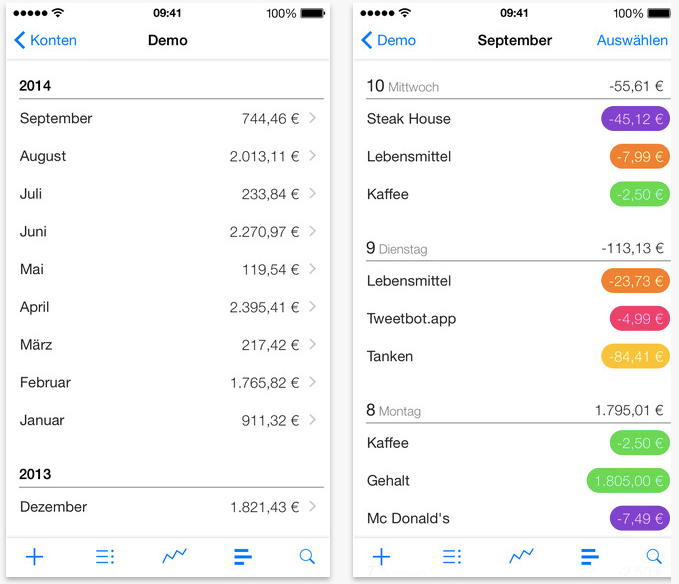
\includegraphics[height=7cm,width=8cm]{meineFinanzen}}
\end{figure}
\clearpage



\subsection{App Moneyboard Pro [2]}
\begin{itemize} 
\item \textbf{Funktionalität}: Moneyboard gibt es für iPhone, iPad und iPod touch. Mit der Finanzapplikation können Einnahmen und Ausgaben verwaltet werden. Transaktionen können nach Woche, Monat oder Jahr gefiltert werden.  Für jede Buchung kann auch ein Belegfoto hinterlegt werden. \\

Im Rahmen eines Gratisversions  kann nur ein Konto mit unbegrenzten Transaktionen festgehalten werden.  Neue Kategorien und Datenexport ist nur im Vollversion möglich.\\\\

\item \textbf{Usability}:\\

\textcolor{green}{\ding{51}}	Konten können mit Profilfoto und Farben individualisiert werden\\
\textcolor{green}{\ding{51}}	Kategorien können mit Symbolbild (icon) veranschaulicht werden\\
\textcolor{green}{\ding{51}}	dynamische Grafiken verstärken die Visualität.\\
\textcolor{red}{\ding{55}}	Sprache: Übersetzung in deutsche Sprache teilweise falsch oder nicht vollständig.\\
\textcolor{red}{\ding{55}}	"Ausgabe" wird auch als Auslage sowie expenses verwendet. \\
\textcolor{red}{\ding{55}}	Schreibfehler (Edigieren statt Redigieren (Korrektur))\\
\end{itemize}


\begin{figure}
\centering
\subfigure[Moneyboard Pro App]{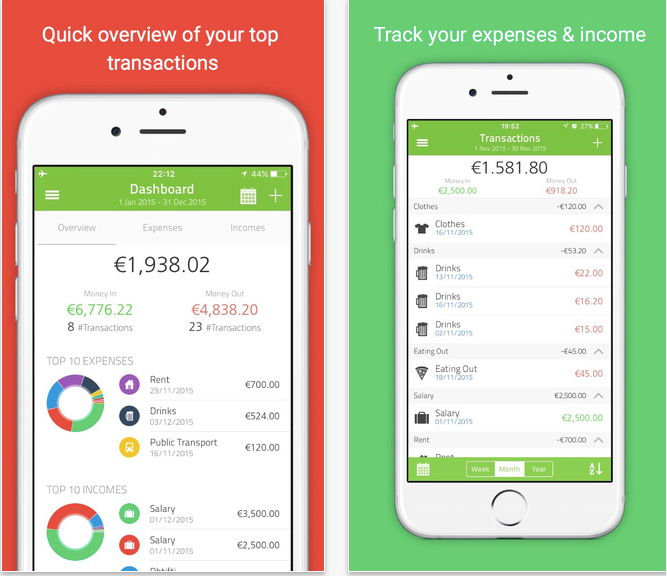
\includegraphics[height=7cm,width=8cm]{moneyboard}}
\end{figure}

\clearpage

\subsection{Haushaltsbuch Pro [3]}
\begin{itemize} 

\item\textbf{Funktionalität}\\
Mit der App gibt es die Möglichkeit ein Haushalt zu erstellen und es mit anderen Nutzern zu teilen, um die Einnahmen und Ausgaben für einen Haushalt gemeinsam zu verwalten. Durch Familien-Synchronisation haben alle Mitglieder des Haushalts Zugriff auf die selben Transaktionen. \\
Im Gratisversion können nur 5 Transaktionen pro Tag erstellt werden. Die App gibt es für iPhone, iPad und iPod touch und bietet auch Apple-Watch App.\\

\item\textbf{Usability}\\

\textcolor{green}{\ding{51}}	Feedback nach Erstellung einer Transaktion\\
\textcolor{green}{\ding{51}}	dynamische Grafiken\\
\textcolor{red}{\ding{55}}	Keine Hilfe-Dokumentation\\

\end{itemize}

\begin{figure}
\centering
\subfigure[HaushaltsPro App]{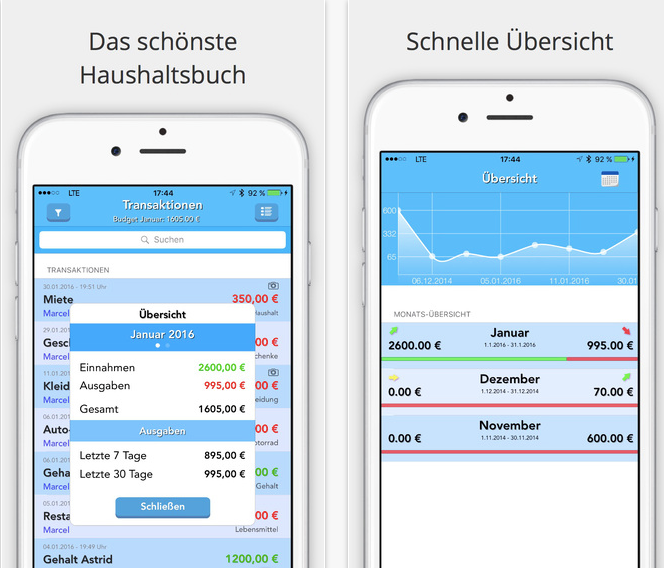
\includegraphics[height=7cm,width=8cm]{haushaltsbuchPro}}
\end{figure}
\clearpage


\subsection{Übersicht der analysierten Applikationen}

\begin{figure}
\centering
\subfigure[Vergleich]{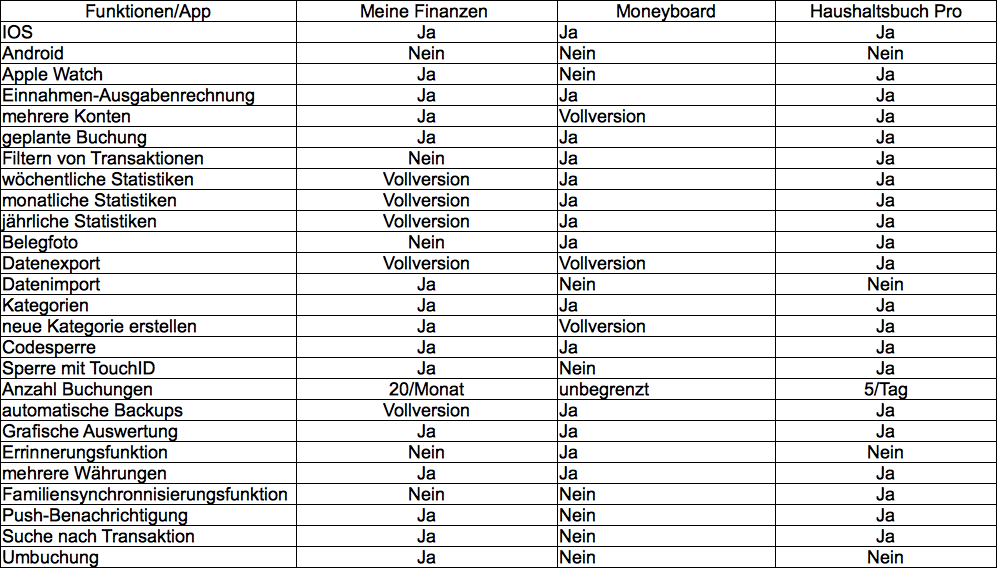
\includegraphics[height=12cm,width=13cm]{ubersicht}}
\end{figure}
\clearpage

\section{Nutzeranalyse (User Analysis)}
\subsection{Übersicht Benutzergruppen}


\textbf{Primär} Erwachsene Personen mit einem durchschnittlichem Einkommen, \\ Familienoberhaupt\\
\textbf{Sekundär} Sachwalter, Buchhalter\\
\textbf{Grenzfälle} Jugendliche unter 16, Ältere Personen über 60\\

\subsection{Beschreibung der Benutzergruppen}

\textbullet \textbf{ Primäre Benutzergruppen}\\
Unsere App wird mit hoher Wahrscheinlichkeit von Erwachsenen Personen, mit einem durchschnittlichen Einkommen, öfters in Anspruch genommen da nun mal für diese Gruppe eine genaue Auflistung, insbesondere der Ausgaben,  sicherlich interessanter ist. Eine kontinuierliche Überwachung der Ein- und Ausgaben kann unter Umständen auf längere Zeit viele unnötige Kosten aufdecken und somit die Lebensqualität, dank einer konkreteren Aufteilung der Finanzen, erheblich steigern.\\
Eine weitere Primäre Nutzergruppe, ungeachtet der Einkommenshöhe, wären Familien-Väter/ Mütter, die die Verantwortung einer gerechten Aufteilung des Einkommens innerhalb des Familienkreises gewährleisten. Auch diese Gruppe würde sicherlich dank der Übersicht welcher unsere App gewährleisten wird sehr profitieren.\\\\

\textbullet\textbf{ Sekundäre Benutzergruppen}\\
Da wir in unserer App, spätestens in den erweiterten Versionen, eine Multiuser Umgebung implementieren werden, so das ein Nutzer auch mehrere Konten verwalten kann, könnte dies die  Interesse bestimmter Berufe wecken, zumal eines Sachwalters. Ein Sachwalter, unter dessen Aufgaben zumeist auch die Verwaltung eines Vermögens fällt, könnte dank unserer App diesen mit Leichtigkeit betreuen und hätte ein Abbild der Ist-Situation immer griffbereit. \\\\
Eine andere Benutzergruppe könnten Buchhalter sein. Natürlich kann unserer App nicht all die umfangreichen Funktionen einer Buchhaltungssoftware abdecken, dennoch wird Sie in der Lage sein die alltäglichen Finanzbewegungen einer Privatperson zur decken.  Dies könnte bei kleinen Einzelunternehmen in der Startphase sicherlich interessant sein. \\


\textbullet \textbf{ Grenzfälle}\\
Da eine "Finanzensteuerung" zumindest einen gewissen Grad an Verantwortungsbewusstsein voraussetzt, ist es weniger zu erwarten, dass Personen unter 16 Jahren, sich für unsere App interessieren. Selbst bei sehr vielen verantwortungsbewussten Jugendlichen, gäbe es wohl aufgrund der eingeschränkten Finanzen trotzdem es keinen Bedarf an unserer App. \\
Bei älteren Personen, insbesondere über 60, denken wir dass der Umstieg von Blatt Papier und Stift selbst bei noch so großartiger "Usability" sehr schwer sein wird. Natürlich wird es auch hier Ausnahmen geben.  


\section{Kontextanalyse}

Wir denken dass unsere App in einer ruhigen Verfassung benutzt wird. Es ist wohl unüblich Finanzen in Hektik zu verwalten. Die Umgebung wird sich allerdings sehr oft ändern. Wir gehen davon aus das die Einnahmen öfters zuhause beziehungsweise auch im Büro eingetragen werden. Die Ausgaben allerdings könnten sehr wohl gleich nach einem Einkauf eingegeben werden. Da dies wahrscheinlich im Stehen oder unterwegs sein wird muss diese Eingabe besonders leicht zu tätigen sein. \\\\Vielleicht wäre angesichts dessen ein Feature, wie zum Beispiel ein "Einkauf getätigt" Button angebracht, welcher zur einen späteren Zeitpunkt die App veranlasst den Nutzer an die unvollständige Aktion zu erinnern. Generell sollte die App eher täglich verwendet werden als ein wöchentlich oder gar monatlich. Ziel sollte es sein jede Bewegung sofort abzubilden. 


\section{Projektmanagement}
\subsection{Kontext}
Entwicklung einer App namens "Meine Finanzen" das die Ein und Ausgaben eines Nutzers abspeichert, kategorisiert und visuell wiedergibt. Entsprechende Berichtsfunktionen, basierend auf Zeitraum und Kategorien, ausgeben und in Bezug auf das Verhalten dynamische Tipps generieren kann.

\subsection{Motivation}
Der Finanzdienstleistungsbereich ist offensichtlich im stark steigenden Trend. Dies liegt insbesondere daran das viele Menschen heutzutage ihr Hauptaugenmerk auf ihre Finanzen richten. Ungeachtet dessen, ob nun richtig oder falsch, ermöglicht dies, im Zusammenhang mit Smartphones welche schon seit längerem ein unverzichtbarer Teil unseres Lebens sind, neue Möglichkeiten. Möglichkeiten diesen Bedarf an Übersicht, sowie an einem dynamischen Ratgeber und eine kontinuierliche Kontrolle der Finanzen durch eine App zu gewährleisten.\\ Unsere Motivation ist es diesen Bedarf abzudecken. Ein Geschäftsmodell können wir uns durch die "Subscriptions"  oder aber auch Free2use im Gegenzug von Austausch von Daten vorstellen. Diese wären dann wiederum, natürlich anonymisiert, für viele Institute interessant. 

\subsection{Ziele}
•	Ein und Ausgaben abbilden\\
•	Budgetierung ermöglichen\\
•	Finance Advisor (Tipps entsprechend Ausgabeverhalten)\\
•	Fertigstellung der App bis 08.06.2016\\


\subsection{Nicht-Ziele}
•	Bankapplikationen zu ersetzten\\
•	Transaktionen durchzuführen (Gelüberweisungen etc.)\\
•	Ausschließlich als ein Ein-Ausgaben Rechner dienen\\



\subsection{Das Projektteam stellt sich vor}
\subsubsection{Ayyildiz Mert Ahmet}
\subsubsection{Bozkurt Yigit Berkay}
\subsubsection{Camkerten Dursun}
\subsubsection{Pektas Tarik}


\clearpage


\section{Personas}
\bigskip
\bigskip
\section{Aufgabenanalyse}
\bigskip
\bigskip
\clearpage

\begin{thebibliography}{1}
\bibitem{proceeding1} https://itunes.apple.com/at/app/meine-finanzen-personliche/id797005152?mt=8
\bibitem{proceeding2}https://itunes.apple.com/us/app/moneyboard-personal-finance/id625887028?mt=8
\bibitem{proceeding3} https://itunes.apple.com/at/app/haushaltsbuch-pro/id879507285?mt=8


\end{thebibliography}


\end{document}